%PDF DI RIFERIMENTO: 03_Requirement Engineering.pdf

\chapter{Requirement Analysis}
    \section{Obiettivo}
        In questa sezione verranno analizzate le informazioni definite nei requisiti di sistema al fine di schematizzare opportunamente il dominio del problema.

    \section{Use Case Diagram}
        %Use Case Diagram costruito con StarUML
        \begin{figure}[htbp!]
            \centering
                \vspace{2\baselineskip}
                \includegraphics[width=0.51\linewidth]{Immagini/Diagrammi/UseCaseDiagram.pdf}
            \caption{Use Case Diagram}
            \label{fig:Use Case Diagram}
        \end{figure}

    \newpage
    
    \section{Target utenti}
        La personas principale scelta è Maria Lombardo. La personas secondaria è Luca Serra
        
        \begin{figure}[!htb]
           \begin{minipage}{0.48\textwidth}
                \centering
             \includegraphics[width=.7\linewidth]{Immagini/Personas/Maria Lombardo.pdf}
             \caption{Maria Lombardo}\label{Fig:Maria Lombardo}
           \end{minipage}\hfill
           \begin{minipage}{0.48\textwidth}
                \centering
             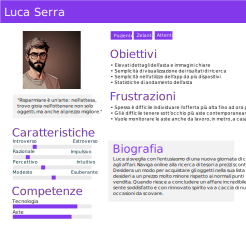
\includegraphics[width=.7\linewidth]{Immagini/Personas/Luca Serra.pdf}
             \caption{Luca Serra}\label{Fig:Luca Serra}
           \end{minipage}
        \end{figure}

        \begin{figure}[!htb]
           \begin{minipage}{0.48\textwidth}
                \centering
             \includegraphics[width=.7\linewidth]{Immagini/Personas/Marco Rossi.pdf}
             \caption{Marco Rossi}\label{Fig:Marco Rossi}
           \end{minipage}\hfill
           \begin{minipage}{0.48\textwidth}
                \centering
             \includegraphics[width=.7\linewidth]{Immagini/Personas/Martina Silvestri.pdf}
             \caption{Martina Silvestri}\label{Fig:Martina Silvestri}
           \end{minipage}
        \end{figure}

        \begin{figure}[!htb]
           \begin{minipage}{0.48\textwidth}
                \centering
             \includegraphics[width=.7\linewidth]{Immagini/Personas/Matteo Luongo.pdf}
             \caption{Matteo Luongo}\label{Fig:Matteo Luongo}
           \end{minipage}\hfill
           \begin{minipage}{0.48\textwidth}
                \centering
             \includegraphics[width=.7\linewidth]{Immagini/Personas/Arturo Campobello.pdf}
             \caption{Arturo Campobello}\label{Fig:Arturo Campobello}
           \end{minipage}
        \end{figure}
        
    \section{Mockup}

    \section{Tabelle di Cockburn}
        \subsection{Crea un’asta inversa}
            \begin{longtable}{|C{3.0cm}|C{1.3cm}|L{5.2cm}|L{5.2cm}|}
                \hline
                    \textbf{USE CASE \#1} &
                    \multicolumn{3}{|l|}{\textbf{Crea un’asta inversa}}\\
                \hline
                    Goal in Context &
                    \multicolumn{3}{|l|}{L'utente di tipo "compratore" vuole creare un'asta inversa.}\\
                \hline
                    Preconditions &
                    \multicolumn{3}{|l|}{L'utente ha effettuato l'accesso con un account di tipo compratore.}\\
                \hline
                    Success End Condition &
                    \multicolumn{3}{|l|}{L'utente di tipo "compratore" ha correttamente creato un'asta inversa}\\
                \hline
                    \multirow[|c|]{5}{*}{DESCRIPTION} 
                    & \textbf{Step n°}
                    & \textbf{Compratore di asta inversa}
                    & \textbf{Sistema}\\
                \cline{2-4}
                        & 1
                        & Preme bottone "Crea asta" su Mockup 6
                        & \\
                \cline{2-4}
                        & 2
                        & 
                        & Mostra Mockup 12 con tutte le informazioni dell'asta da poter inserire.\\
                \cline{2-4}
                        & 3
                        & Preme sul campo di input "Data di scadenza"
                        & \\
                \cline{2-4}
                        & 4
                        & 
                        & Mostra il pannello di selezione della data da calendario\\
                \cline{2-4}
                        & 5
                        & Seleziona la data
                        & \\
                \cline{2-4}
                        & 6
                        & Clicca su OK
                        & \\
                \cline{2-4}
                        & 7
                        & Preme sul campo di input "Ora di scadenza"
                        & \\
                \cline{2-4}
                        & 8
                        & 
                        & Mostra il pannello di selezione dell'ora\\
                \cline{2-4}
                        & 9
                        & Seleziona l'ora
                        & \\
                \cline{2-4}
                        & 10
                        & Clicca su OK
                        & \\
                \cline{2-4}
                        & 11
                        & Preme sul campo di input "Prezzo di partenza"
                        & \\
                \cline{2-4}
                        & 12
                        &
                        & Mostra il tastierino numerico \\
                \cline{2-4}
                        & 13
                        & Inserisce il prezzo di partenza
                        & \\
                \cline{2-4}
                        & 14
                        & Preme sul campo di input "Nome prodotto"
                        & \\
                \cline{2-4}
                        & 15
                        &
                        & Mostra la tastiera \\
                \cline{2-4}
                        & 16
                        & Inserisce il nome del prodotto oggetto dell'asta
                        & \\
                \cline{2-4}
                        & 17
                        & Preme sul campo di input "Categoria"
                        & \\
                \cline{2-4}
                        & 18
                        &
                        & Mostra il menù a tendina con le diverse categorie tra cui scegliere \\
                \cline{2-4}
                        & 19
                        & Seleziona la categoria
                        & \\
                \cline{2-4}
                        & 20
                        & Preme sul campo di input "Descrizione"
                        & \\
                \cline{2-4}
                        & 21
                        &
                        & Mostra la tastiera \\
                \cline{2-4}
                        & 22
                        & Inserisce la descrizione del prodotto oggetto dell'asta
                        & \\
                \cline{2-4}
                        & 23
                        & Preme sul pulsante "Crea"
                        & \\
                \cline{2-4}
                        & 24
                        & 
                        & Mostra Mockup X (Schermata di successo)\\
                \hline
                    EXTENSIONS
                    & \textbf{Step n°} 
                    & \textbf{Compratore di asta inversa} 
                    & \textbf{Sistema}\\
                \hline
                    \multirow[|c|]{3}{*}{\shortstack[c]{Seleziona ora \\ antecedente a \\quella attuale (la\\ data è quella\\ attuale)}}
                        & 11.a
                        & 
                        & Mostra Mockup Y con testo "Non puoi selezionare un'ora antecedente a quella attuale"\\
                \cline{2-4}
                        & 12.a
                        & Clicca su OK
                        & \\
                \cline{2-4}
                        & 13.a
                        & 
                        & Continua da step 7 di main scenario\\
                \hline
                    \multirow[|c|]{3}{*}{\shortstack[c]{Seleziona prezzo di \\ partenza negativo}}
                        & 14.b
                        & 
                        & Mostra Mockup P24 con testo "Non puoi inserire un prezzo di partenza negativo"\\
                \cline{2-4}
                        & 15.b
                        & Clicca su OK
                        & \\
                \cline{2-4}
                        & 16.b
                        & 
                        & Continua da step 11 di main scenario\\
                \hline
                    \multirow[|c|]{2}{*}{\shortstack[c]{Alcuni campi \\ obbligatori non \\ compilati}}
                        & 24.c
                        & 
                        & Mostra Mockup E11 dove vengono segnalati in rosso i campi obbligatori non compilati\\
                \cline{2-4}
                        & 25.c
                        & Riparte da step 3 di main scenario, saltando i campi di input già compilati
                        & \\
                \hline
                    \multirow[|c|]{4}{*}{\shortstack[c]{Esce dalla pagina \\ di creazione asta}}
                        & \textit{In qualunque passo del main scenario}
                        & Preme qualsiasi tasto di navigazione (della navbar in basso o tasto "indietro")
                        & \\
                \cline{2-4}
                        & 
                        & 
                        & Mostra Mockup Z con testo "Sei sicuro di voler uscire dalla creazione asta? I dati inseriti andranno persi." \\
                \cline{2-4}
                        & 
                        & Clicca su OK
                        & \\
                \cline{2-4}
                        & 
                        & 
                        & Mostra Mockup corrispondente al tasto cliccato\\
                \hline
                    SUBVARIATIONS
                    & \textbf{Step n°} 
                    & \textbf{Compratore di asta inversa} 
                    & \textbf{Sistema}\\
                \hline
                    \multirow[|c|]{5}{*}{\shortstack[c]{Inserisce immagine}}
                        & 14.s1
                        & Preme sul campo di input "Aggiungi immagine prodotto"
                        & \\
                \cline{2-4}
                        & 15.s1
                        & 
                        & Mostra il sistema per selezionare le immagini\\
                \cline{2-4}
                        & 16.s1
                        & Seleziona una o più immagini
                        & \\
                \cline{2-4}
                        & 16.s1
                        & Clicca su OK
                        & \\
                \cline{2-4}
                        & 17.s1
                        & 
                        & Continua da step 14 di main scenario\\
                \hline
            \end{longtable}